\documentclass{article}
\usepackage{graphicx}
\usepackage[margin=1.5in]{geometry}
\usepackage{hyperref}

\title{Homework \#1: Recipe}
\author{CSCI 342, Fall 2017}

\begin{document}

\maketitle



\paragraph{Description:}
  This assignment tests your understanding of basic HTML and CSS. You
will create several files related to a recipe web site for a fictional
pie company named Granny's Pies. Turn in the following files:
\begin{itemize}
\item \verb|index.html|, the first of two web pages (with an optional
  CSS style sheet file); appearance is up to you
\item \verb|index.css|, an optional style file for \verb|index.html|.
\item \verb|pie.html|, the second of two web pages; must match a
  particular specified appearance
\item \verb|recipe.css|, the style sheet for \verb|pie.html|
\end{itemize}
For full credit, your files must be zipped together into a file named
\verb|csci342hw01.zip| and uploaded to canvas before the deadline, and
must match the guidelines in this document.  Make sure you zip {\em
  just the files} and not the folder containing the files. This is so
I can run a script to unzip everything and run some tests without my
interaction.

\paragraph{Due date:} Friday, October 20, midnight.


\paragraph{Index Page:} The first part of your task is to create a front
  page for this web site, stored in a file named
  \verb|index.html|. Your front page must contain a link to
  \verb|pie.html|. The file must also be at least 20 lines long and
  must contain at least 4 different HTML elements in its body. It also
  may not significantly borrow content from your
  \verb|pie.html|. Otherwise, this front page can have any appearance
  you like. If you like, you may use an optional CSS file with this
  page named \verb|index.css| and submit it with your other files. Be
  creative! We may show some students' pages in class.

\paragraph{Pie Recipe Page:} The second part is to recreate a specific web
  page of a recipe for lemon meringue pie, stored in a file named
  \verb|pie.html|. Unlike \verb|index.html|, this page must exactly
  match the appearance specified in this document.  You must match in
  appearance the pie web page shown in the Figure \ref{piefigure}.

  Based on browser, operating system, and other factors, your page may
  not exactly match fonts and colors, but they should approximate them. The
  width of your page will also alter the line breaks, which are
  done automatically by the browser, except ones that are clearly
  much narrower than the page width, such as the line ``One 9-inch
  pie.''


\paragraph{Provided Output Text:} You don't need to type in all of the text
  of the pie web page, only the HTML tags. There is a provided text
  file on the course web site that you can copy and paste into your
  text editor to get started. Then you can add the appropriate HTML
  tags to the file and save it as your \verb|.html| page.

\paragraph{Appearance and Behavior Details:}\mbox{}
  \begin{itemize}
    \item The pie web page's title text
      should be {\bf Grandma's Lemon Meringue Pie}.
    \item All headings on the page should use a foreground color of
      {\tt \#A4A400} (red=164, green=164, blue=0) and a background color of
      {\tt \#F0F0F0} (red=240, green=240, blue=240).
    \item The font families for headings are: Lucida Sans Unicode,
      Helvetica, Arial, or any sans-serif font available on the system
      (in that order).
    \item The page's main heading is aligned to the center of the page
      body, and uses a 22pt bold font.
    \item Other headings on the page are
      leftaligned and appear in an 18pt normal font.
    \item All headings
      should be underlined.
    \item The overall page's body should have a
      white background.
    \item Text in the body should have a foreground
      color of {\tt \#404040} (red=64, green=64, blue=64) and use an 11pt
      font.
    \item The font families for page text are Georgia, Garamond, or
      any serif font available on the system.
    \item Any links on the page
      should use the color {\tt \#A4A400} (red=164, green=164, blue=0),
      matching the color of the page headings.
    \item In the Ingredients
      list, the underlined words ``tbsp'' and ``tsp'' are abbreviations
      for ``tablespoons'' and ``teaspoon'' respectively. When the user
      hovers the mouse over these abbreviations, the full word should
      appear as a tooltip.
    \item At the end of the Directions, the deleted
      word ``cake'' with a strike-out line through it is replaced by the
      word ``pie''.
    \item After the Links section there is a short copyright
      notice that appears as a section of pre-formatted text in a
      monospace font. The text is spaced such that the last letter
      lines up horizontally for each of the three lines.
    \item The names of the four major steps of the recipe directions
      (such as ``Preheat Oven'') are strongly emphasized.
    \item The quotations from the users appear in an italic font as
      indented blocks with background color {\tt \#FFFFA8} (red=255,
      green=255, blue=168). Some words in the last quote are bolded
      for emphasis.
    \item The picture of the pie is from the file {\tt pie.jpg}
      provided on the homework website.
    \item The ``Home'' link should go to
      your \verb|index.html| page. Use a relative URL and assume it is
      located on the same site and directory as \verb|pie.html|.
    \item The
      ``Search for other lemon meringue pie recipes'' text
      should link to \\
      \url{http://www.google.com/search?q=lemon+meringue+pie+recipe&start=10}
    \item The ``W3C HTML5'' button, and ``W3C CSS'' button should
      link to the validation web pages as explained here:
      \url{https://validator.w3.org/docs/help.html#manual}.
      
      Note: these links {\em will not work} when you open the html
      file in a browser, but should work when the pages are served
      by a web server.  Since we're not using servers yet, don't
      worry about this, just copy and paste the suggested code from
      the above website.
      
      To validate your pages without serving them, use the file
      upload or copy and paste method of the validation service.
      
    \item All other decisions about styling on the page are left to
      the web browser. Any styles mentioned previously that are the
      same as browser defaults do not have to be explicitly included
      in your CSS style sheet. The screenshot in this document was
      taken on Linux using Chrome, which may differ from the
      appearance on your system.
  \end{itemize}
      
\paragraph{Extra Features:} In addition to the previous required features,
  you must also complete at least two (2) of the following additional
  requirements in your pie page. These are features that may have not
  been covered in detail in lecture; you will have to explore 
  online resources to learn how to complete these features. If you want to
  complete more than two of the extra features below, that is fine,
  but only two are required.
  \begin{itemize}
  \item {\bf Background:}  Set the overall page to use a background image of:
    {\tt silverware.jpg}. The image should repeat in both directions
    across the page and should not move when the page is scrolled.
  \item {\bf Favicon:}  Set the page to have a ``favorites icon''
    (``favicon''). Use: {\tt pie-icon.gif} The icon may not work in
    Internet Explorer; you may ignore this.
  \item {\bf Pie bullet:}  Set all bulleted lists of items on the page to use
    an image for their bullet icon rather than the normal black
    circle. Use the following image: {\tt pie-icon.gif}
  \item {\bf Wide headings:}  Place 0.25em horizontal spacing between
    neighboring letters in all headings on the page.
  \item {\bf Tight heading background:}  Make it so that the gray background
    behind the headings on the page is only behind the text itself,
    not stretched across the entire width of the page. (Looks nice
    with extra feature \#1.)
  \item {\bf Other:}  Do you have an extra feature you'd like to add to
    your page that isn't listed here? Ask me and I'll let you know if
    it is okay to substitute for one of the above.
  \end{itemize}
  Near the top of your HTML file, put a comment saying which extra
  features you have completed.  As much as possible, you should
  implement these changes by modifying your CSS code rather than your
  HTML.  Some of the CSS properties necessary will not have been
  covered in class, so you must learn them yourself.


\paragraph{Implementation and Grading:} \mbox{}
  \begin{itemize}
    \item For full credit, your pie.html page must pass the W3C HTML5
      validator with no errors (a green bar). (Your page is fine as
      long as you see the green bar and text ``Document checking
      completed. No errors or warnings to show.'')
    \item Choose appropriate HTML tags to match the structure of the
      content on the page. Do not express style information in HTML
      with inline styles or presentational HTML tags such as b or
      font.
    \item You may not use any HTML tables in your pie.html page.
    \item You only need to worry about your page's appearance in
      standards-compliant browsers such as Firefox or Chrome.  You
      will not be tested in Microsoft Internet Explorer or other
      browsers that do not comply to web standards.
    \item Express all stylistic information on the page using CSS
      defined in {\tt recipe.css}. For full credit, your style sheet
      must successfully pass the W3C CSS validator.
    \item Part of your grade comes from expressing your CSS concisely
      and without unnecessary or redundant styles. For example, if the
      page uses the same color or font family for multiple elements on
      the page, you must group those elements into a single CSS rule,
      so that it would be possible to change the page's color/font by
      modifying a single place in the CSS file.
    \item Outside of extra features, do not use HTML or CSS constructs
      that have not been discussed in lecture or the slides.
    \item Do not overuse HTML class and id attributes to target
      elements for styling. If there is already a suitable tag for
      representing a given piece of content, favor the use of that tag
      rather than a less appropriate tag with a class or id attached
      for styling purposes.
    \item Format your HTML and CSS nicely so that
      it is as readable as possible, similarly to the examples shown
      in class.
    \item Also place a comment header in each file containing your
      name, the course name and number, and a brief description of the
      assignment and the file's contents.
    \item You must properly use whitespace and indent your HTML and
      CSS code following examples shown in class.
    \item To keep line lengths
      manageable, do not place more than one block element on the same
      line or begin any block element past the 100th character on a
      line.
    \item The majority of the points for this assignment will be for
      the \verb|pie.html| and its \verb|recipe.css| files.  The
      \verb|index.html| will also be graded, but it will be worth
      fewer points.
    \item The main stylistic constraint on your
      \verb|index.html| file is that it should pass the W3C HTML5 and
      CSS validators. Beyond that it can contain any non-obscene
      content you like, even content that uses material we have not
      yet learned in lecture.
    \item Please do not link to external resources from your
      {\tt index.html} page, other than the image files and the
      resources specified in the requirments, above.
    \item Submit your assignment online on canvas.
    \item Zip together all files, including images, so that the
      website is complete upon unzipping.  Do not zip the folder:
      after unzipping the files should be in the same folder as the
      zip file.
    \item Include any extra images you used in the zip file.
    \item If you used any absolute links to resources, you do not have
      to include local copies of them.
    \item Part of your grade will come from correctly zipping and
      successfully uploading your solution to canvas.
  \end{itemize}
  

\begin{figure}
  \begin{center}
    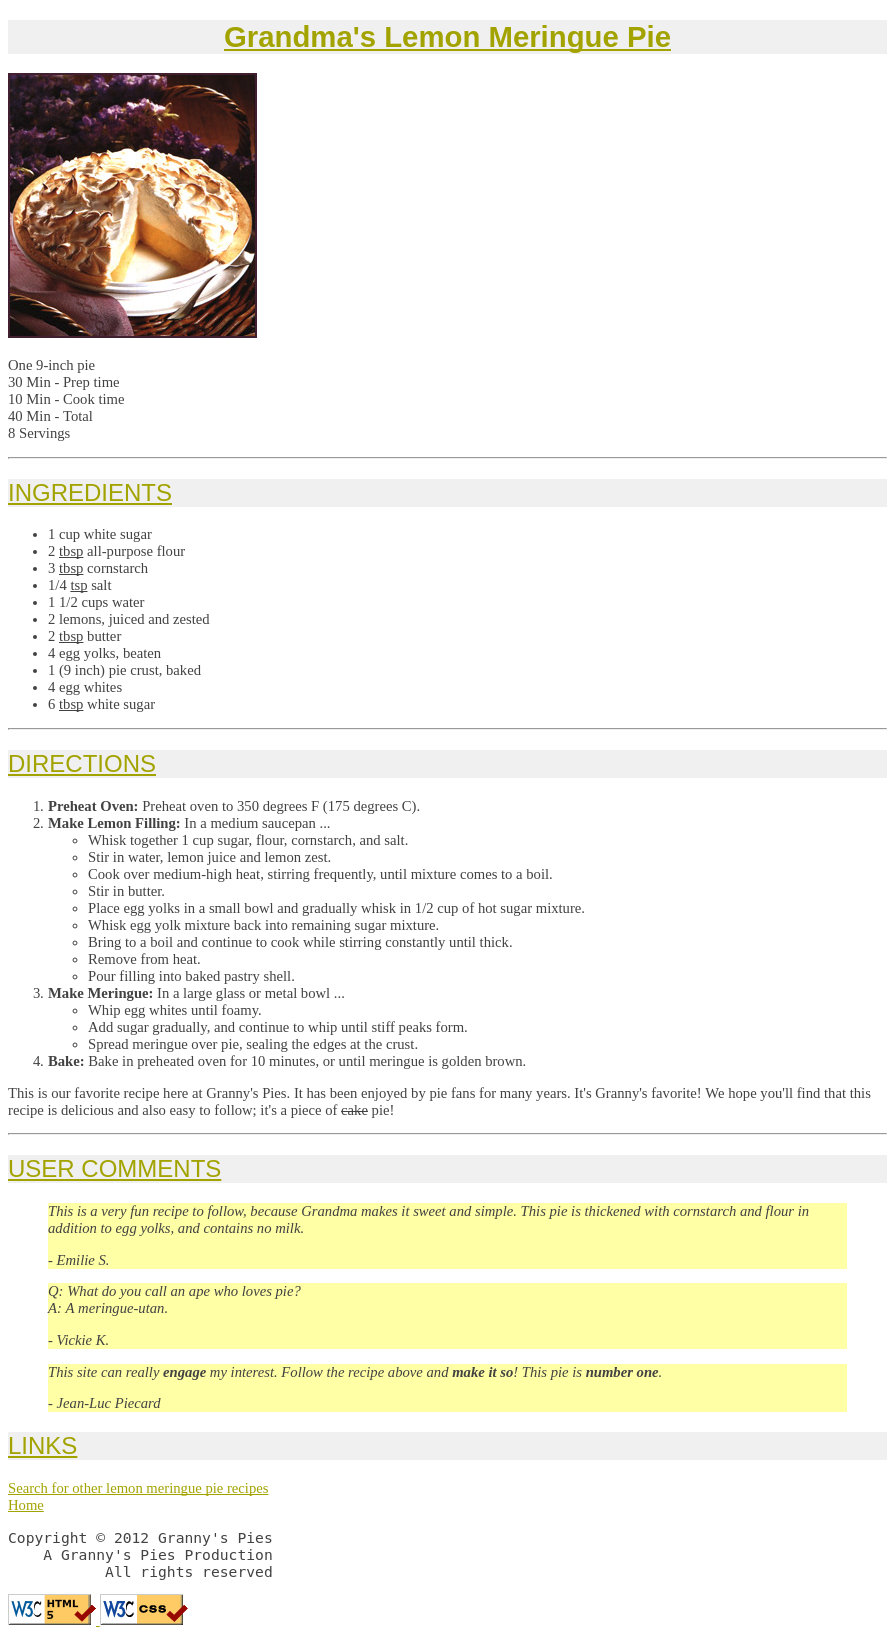
\includegraphics[height=0.9\textheight]{grandma.png}
  \end{center}
  \caption{Desired appearance of {\tt pie.html}.  Small differences
  depending on browser/system/{\em etc.} are acceptable.  This was
  made using Chrome on Linux.}
\label{piefigure}
\end{figure}

\paragraph{Acknowledgements:} This assignment is adapted from one that is:
Copyright \copyright Marty Stepp / Jessica Miller, licensed under
\href
    {https://creativecommons.org/licenses/by/2.5/}
    {Creative Commons Attribution 2.5 License}.
    All rights reserved.


\end{document}
